\documentclass[../../../../main.tex]{subfiles}
\begin{document}

\section*{第1問}

\begin{proof}[解]
(i) (イ) 全て \quad (ロ) 少なくとも \quad (ハ) ない

\bigskip
(ii) まず A が A' に一致するように平行移動する．
次に，A を中心に BC が B'C' と同一線上にあるように回転移動する．これで $\triangle ABC$ と $\triangle A'B'C'$ が一致しなければ，A を通り BC に垂直な直線を軸に線対称移動する．

\bigskip
(iii) 完全に一致するとすると，任意の $x, h$ に対し
\[
  f(x+h) = f(x)
\]
が成立する．
\begin{align*}
  &(x+h)^4 + a(x+h)^3 + b(x+h)^2 + c(x+h) + d \\
  &= x^4 + ax^3 + bx^2 + cx + d \\
  \iff &(4h x^3 + 6h^2 x^2 + 4h^3 x + h^4) + a(3h x^2 + 3h^2 x + h^3) + b(2hx + h^2) + ch = 0
\end{align*}
$3$ 次の項を比較して $4h = 0$ だが $h \neq 0$ に反し矛盾．
よって示された．
\end{proof}

\newpage

\section*{第2問}

\begin{proof}[解]
\begin{center}
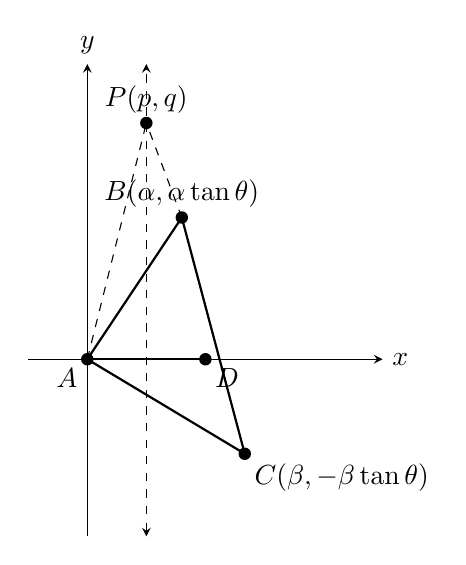
\begin{tikzpicture}[scale=1.5, >=stealth]
  \draw[->] (-0.5,0) -- (2.5,0) node[right] {$x$};
  \draw[->] (0,-1.5) -- (0,2.5) node[above] {$y$};
  \node[below left] at (0,0) {$A$};
  \coordinate (A) at (0,0);
  \coordinate (D) at (1,0);
  \node[below right] at (1,0) {$D$};
  
  \coordinate (B) at (0.8, 1.2);
  \coordinate (C) at (1.333, -0.8);
  \coordinate (P) at (0.5, 2.0);
  
  \draw[line width=0.8pt] (A) -- (B) -- (C) -- cycle;
  \draw[line width=0.8pt] (A) -- (D);
  \draw[dashed] (B) -- (P);
  \draw[dashed] (A) -- (P);
  \draw[<->, dashed] (0.5,-1.5) -- (0.5,2.5);
  
  \node[above] at (B) {$B(\alpha, \alpha\tan\theta)$};
  \node[below right] at (C) {$C(\beta, -\beta\tan\theta)$};
  \node[above] at (P) {$P(p,q)$};
  
  \fill (A) circle (1.5pt);
  \fill (D) circle (1.5pt);
  \fill (B) circle (1.5pt);
  \fill (C) circle (1.5pt);
  \fill (P) circle (1.5pt);
\end{tikzpicture}
\end{center}

$AD=1$ として一般性を失わない．A を原点とし，AD を $x$ 軸とする上図のような座標平面をとり
\[
  B(\alpha, \alpha \tan \theta) \quad \left(0 < \theta < \frac{\pi}{2}\right)
\]
\[
  C(\beta, -\beta \tan \theta)
\]
とおく ($\alpha \neq \beta$, $\alpha, \beta > 0$)．
\begin{align*}
  BC: &(\beta + \alpha)\tan \theta \cdot (x - \alpha) + (\beta - \alpha)(y - \alpha \tan \theta) = 0 \\
  &(\beta + \alpha)\tan \theta \cdot x + (\beta - \alpha)y - 2\alpha\beta \tan \theta = 0 \quad \dots \text{①}
\end{align*}
これが $D(1,0)$ を通るので
\[
  (\beta + \alpha)\tan \theta = 2\alpha\beta \tan \theta
\]
$\tan \theta \neq 0$ より
\[
  \alpha + \beta = 2\alpha\beta \quad \dots \text{②}
\]

$\triangle ABC$ の外心 $O'(X,Y)$ とすると，$O'A = O'B = O'C$ から
\begin{align}
  X &= \frac{1}{4}(\tau^2 + 1)(\alpha + \beta) \quad \dots \text{③} \quad (\tau = \tan \theta) \\
  Y &= \frac{1}{4\tau}(\tau^2 + 1)(\alpha - \beta) \quad \dots \text{④}
\end{align}
となり，外接円は $C: (x-X)^2 + (y-Y)^2 = X^2 + Y^2$ だから点 A での接線 $l$ は
\begin{align*}
  l: &Xx + Yy = 0 \\
  &(\alpha + \beta)\tau x + (\alpha - \beta)y = 0 \quad \dots \text{⑤}
\end{align*}

よって ①, ⑤ から BC と $l$ の交点 $P(p,q)$ は
\[
  p = \frac{1}{2}, \quad q = \frac{\alpha + \beta}{\beta - \alpha} \frac{\tau}{2}
\]
よって P は定直線 $x = \dfrac{1}{2}$ 上にあるから示された．

\bigskip
\begin{proof}[別解]
\begin{center}
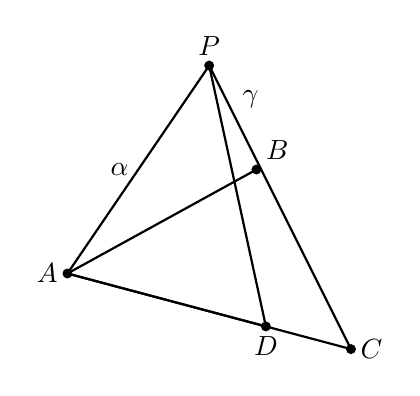
\begin{tikzpicture}[scale=1.2, >=stealth]
  \coordinate (P) at (1.5, 3.0);
  \coordinate (A) at (0, 0.8);
  \coordinate (C) at (3.0, 0);
  \coordinate (B) at (2.0, 1.9);
  \coordinate (D) at (2.1, 0.24);
  
  \draw[line width=0.8pt] (A) -- (P) -- (C) -- cycle;
  \draw[line width=0.8pt] (A) -- (B);
  \draw[line width=0.8pt] (P) -- (D);
  \draw[line width=0.8pt] (A) -- (D);
  
  \node[above] at (P) {$P$};
  \node[left] at (A) {$A$};
  \node[right] at (C) {$C$};
  \node[above right] at (B) {$B$};
  \node[below] at (D) {$D$};
  
  \node[left] at (0.75, 1.9) {$\alpha$};
  \node[above right] at (1.75, 2.45) {$\gamma$};
  
  \fill (A) circle (1.5pt);
  \fill (B) circle (1.5pt);
  \fill (C) circle (1.5pt);
  \fill (D) circle (1.5pt);
  \fill (P) circle (1.5pt);
\end{tikzpicture}
\end{center}

$AP = \alpha$, $AB = \beta$, $BP = \gamma$ とおく．
$\triangle ABP \sim \triangle CAP$ より
\[
  AC = \frac{\alpha}{\gamma}\beta \quad \dots \text{①}
\]
又，$\alpha^2 = \gamma \cdot PC$ から
\[
  PC = \frac{\alpha^2}{\gamma} \quad \dots \text{②}
\]
従って
\[
  BD = BC \cdot \frac{AB}{AB+AC} = \left(\frac{\alpha^2}{\gamma} - \gamma\right) \frac{\beta}{\beta + \frac{\alpha}{\gamma}\beta} = \alpha - \gamma
\]
から $DP = PB + BD = \gamma + (\alpha - \gamma) = \alpha$ だから $\triangle APD$ は 2 等辺三角形．
よって P は AD の垂直2等分線上にある．
\end{proof}
\end{proof}

\newpage

\section*{第3問}

\begin{proof}[解]
$M$ を原点，$AB$ を $x$ 軸，$MP$ を $y$ 軸とする右のような座標をとる（対称性から $Q$ が第 1 象限にあるとしてよい）．

\begin{center}
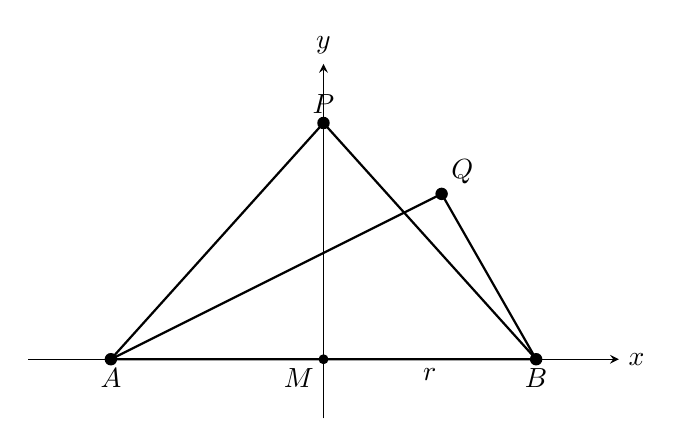
\begin{tikzpicture}[scale=1.5, >=stealth]
  \draw[->] (-2.5,0) -- (2.5,0) node[right] {$x$};
  \draw[->] (0,-0.5) -- (0,2.5) node[above] {$y$};
  
  \coordinate (M) at (0,0);
  \coordinate (A) at (-1.8,0);
  \coordinate (B) at (1.8,0);
  \coordinate (P) at (0,2.0);
  \coordinate (Q) at (1.0, 1.4);
  
  \draw[line width=0.8pt] (A) -- (P) -- (B) -- cycle;
  \draw[line width=0.8pt] (A) -- (Q) -- (B);
  
  \node[below left] at (M) {$M$};
  \node[below] at (A) {$A$};
  \node[below] at (B) {$B$};
  \node[above] at (P) {$P$};
  \node[above right] at (Q) {$Q$};
  
  \node[below] at (0.9,0) {$r$};
  
  \fill (M) circle (1.2pt);
  \fill (A) circle (1.5pt);
  \fill (B) circle (1.5pt);
  \fill (P) circle (1.5pt);
  \fill (Q) circle (1.5pt);
\end{tikzpicture}
\end{center}

\[
  Q\left(a \sin\left(\frac{\pi}{2}-\theta\right), a \cos\left(\frac{\pi}{2}-\theta\right)\right) = Q(a \sin\theta, a \cos\theta)
\]

\begin{enumerate}[(1)]
  \item $\tan \dfrac{\alpha}{2} = t$ とおくと $t = \dfrac{r}{a}$ だから
  \[
    \tan \alpha = \frac{2t}{1-t^2} = \frac{2(r/a)}{1-(r/a)^2} = \frac{2ra}{a^2-r^2}
  \]

  \item $\vec{QA} = \begin{pmatrix} -r - a \sin\theta \\ -a \cos\theta \end{pmatrix}$, $\vec{QB} = \begin{pmatrix} r - a \sin\theta \\ -a \cos\theta \end{pmatrix}$ から
  \begin{align*}
    \tan \beta &= \frac{|\vec{QA} \cdot \vec{QB} \cdot \sin\beta|}{\vec{QA} \cdot \vec{QB}} \\
    &= \frac{|(-r - a s)(-a c) - (r - a s)(-a c)|}{(r - a s)(-r - a s) + a^2 c^2} \quad (c = \cos\theta, s = \sin\theta) \\
    &= \frac{|2 r a c|}{a^2 - r^2} = \frac{2 r a c}{a^2 - r^2} \quad (\because 2 r a c > 0)
  \end{align*}
  だから
  \[
    \tan \alpha \cdot c = \frac{2 r a c}{a^2 - r^2} = \tan \beta
  \]
  である．
\end{enumerate}
\end{proof}

\newpage

\section*{第4問}

\begin{proof}[解]
出発点の座標を $0$ とすると時刻 $t$ での A, B の座標は各々
\[
  A \dots a t
\]
\[
  B \dots v\left(t - \frac{l}{a}\right) \quad \left(t \ge \frac{l}{a}, v > a\right)
\]
とおける．B が A に追いつく時刻 $t_0$ は
\[
  t_0 = \frac{l/a}{1 - \frac{a}{v}} = \frac{l v}{a(v-a)}
\]
である．したがって，B のひろう $f(v)$ は
\begin{align*}
  f(v) &= v^2 \left(t_0 - \frac{l}{a}\right) \\
  &= \frac{v^2}{v-a} l = l \left(v + a + \frac{a^2}{v-a}\right)
\end{align*}
\[
  \frac{f'(v)}{l} = 1 - \frac{a^2}{(v-a)^2} = \frac{v(v-2a)}{(v-a)^2}
\]
以下表を考える．

\[
\begin{array}{c|c*3{c}}
v & a & \dots & 2a & \dots \\ \hline
f' & & - & 0 & + \\ \hline
f & & \searrow & & \nearrow
\end{array}
\]

よって $v = 2a$ の時，疲労が最小．
\end{proof}

\newpage

\section*{第5問}

\begin{proof}[解]
・ $n \le 1$ の時 $S = \sum_{k=1}^{100} (k-n) = \frac{1}{2} \cdot 100 \cdot 101 - 100 n$ から $S$ は $n$ について単調減少．

・ $n \ge 100$ の時 $S = \sum_{k=1}^{100} (n-k) = 100 n - \frac{1}{2} \cdot 100 \cdot 101$ から $S$ は $n$ について単調増加．

よって $1 \le n \le 99$ で考える ($S|_{n=99} < S|_{n=100}$)．
\begin{align*}
  S &= \sum_{k=1}^n (n-k) + \sum_{k=n+1}^{100} (k-n) \\
  &= n^2 - \frac{1}{2} n(n+1) + \frac{1}{2}(101-n)(100-n) \\
  &= n^2 - \frac{1}{2} n - \frac{1}{2} \cdot 201 n + 50 \cdot 101 \\
  &= n^2 - 101 n + 50 \cdot 101 \\
  &= \left(n - \frac{101}{2}\right)^2 + 50 \cdot 101 - \frac{101^2}{4}
\end{align*}
よって $n = 50, 51$ の時 $\min S = 2500$ となる．
\end{proof}

\newpage

\section*{第6問}

\begin{proof}[解]
A の出発点を $0$ とする．時刻 $t$ での A, B の位置 $f(t), g(t)$ とすると
\begin{align*}
  f(t) &= \int_0^t (p^2 + 5) dp = \frac{1}{3} t^3 + 5t \\
  g(t) &= 2 + \int_0^t 5p dp = \frac{5}{2} t^2 + 2
\end{align*}
だから $0 \le t \le 4$ で $f(t) = g(t)$ となる $t$ の数を求めればよい．
$h(t) = f(t) - g(t)$ とおくと，これは $h(t) = 0$ となる $t$ の数にひとしい．

\begin{align*}
  h'(t) &= t^2 + 5 - 5t \\
  &= \left(t - \frac{5-\sqrt{5}}{2}\right)\left(t - \frac{5+\sqrt{5}}{2}\right)
\end{align*}
から下表をえる．

\[
\begin{array}{c|c*5{c}|c}
t & 0 & \dots & \frac{5-\sqrt{5}}{2} & \dots & \frac{5+\sqrt{5}}{2} & \dots & 4 \\ \hline
h' & & + & 0 & - & 0 & + & \\ \hline
h & -2 & \nearrow & & \searrow & & \nearrow & -\frac{2}{3}
\end{array}
\]

ここで $h(t) = \left(\frac{1}{3}t - \frac{5}{6}\right) h'(t) - \frac{5}{6}t + \frac{13}{6}$ から
\begin{align*}
  h\left(\frac{5-\sqrt{5}}{2}\right) &= \frac{1}{12}(1 + 5\sqrt{5}) > 0 \\
  h\left(\frac{5+\sqrt{5}}{2}\right) &= \frac{1}{12}(1 - 5\sqrt{5}) < 0
\end{align*}
だから求める $t$ は 2個 である．
\end{proof}

\end{document}
